\chapter{身边的声音}\label{ch:g3:sound-around-us}

哼一哼你最喜欢的歌 —— 哼的时候，用两根手指轻轻
按住喉咙的前面。感觉到颤动了吗？你刚刚
就摸到了\omterm{def:g3:sound-around-us:sound}{声音}的诞生之处。每一种\omterm{def:g3:sound-around-us:sound}{声音}、每一面鼓、
每一扇吱呀作响的门，发出\omterm{def:g3:sound-around-us:sound}{声音}的方式都完全相同，
本章就来找出其中的窍门。

\section{声音从哪里来}

\begin{definition}[振动]\label{def:g3:sound-around-us:vibration}
称\emph{振动}\index{振动}为非常快速的颤动——
即每秒内多次重复的来回运动，
往往快得让人眼无法跟上。拨动的吉他弦会振动：你
只能看到一片模糊，但指尖能感觉到嗡嗡的震颤。
\end{definition}

\begin{definition}[声音]\label{def:g3:sound-around-us:sound}
称\emph{声音}\index{声音}为当某个物体\omterm{def:g3:sound-around-us:vibration}{振动}，
其颤动通过\omterm{def:g2:air-around-us:air}{空气}传到我们耳中时，我们听到的东西。
发出\omterm{def:g3:sound-around-us:vibration}{振动}的物体是声音的\emph{声源}——一根弦、一张鼓面、
一只铃铛，或你自己的喉咙。
\end{definition}

\begin{method}[让米粒跳舞]\label{met:g3:sound-around-us:rice}
要\emph{看见}\omterm{def:g3:sound-around-us:sound}{声音}是怎样产生的：
\begin{enumerate}
  \item 在鼓面上撒几粒米（也可以撒在铁罐的塑料盖上，
        或绷紧的气球皮上）；
  \item 敲击米粒附近的鼓面——“咚”！米粒跳起来了！
  \item 现在只需离鼓面很近，对着它\emph{大喊}：米粒
        又会颤动起来，即使没有被碰到。
\end{enumerate}
只要鼓面发声，它就在\omterm{def:g3:sound-around-us:vibration}{振动}——即使是从你嘴里传来的\omterm{def:g3:sound-around-us:sound}{声音}，
也会使它颤动。
\end{method}

\begin{omfigure}
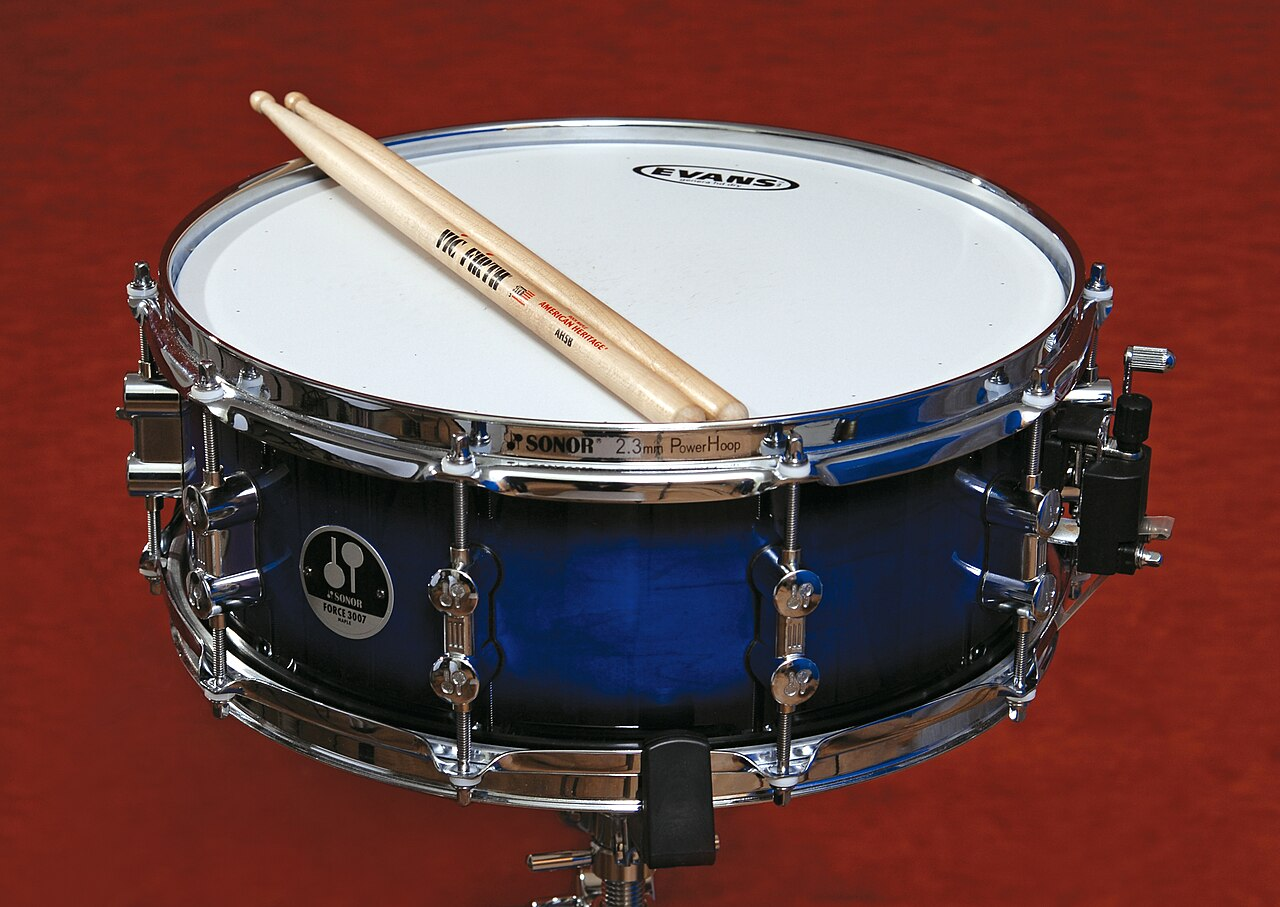
\includegraphics[width=0.58\linewidth]{images/book1/drum.jpg}

{\small 米粒实验用的真鼓：白色的部分是
会颤动的鼓面。在上面撒几粒米，敲击米粒附近——
会发声的鼓面就是会颤动的鼓面，米粒跳舞正说明这一点。
\emph{照片：Vladimir Morozov，CC BY 2.0。}}
\end{omfigure}

\begin{proposition}[没有振动，就没有声音]\label{prop:g3:sound-around-us:novib}
每一种\omterm{def:g3:sound-around-us:sound}{声音}都来自\omterm{def:g3:sound-around-us:vibration}{振动}——\omterm{def:g3:sound-around-us:vibration}{振动}一旦停止，
\omterm{def:g3:sound-around-us:sound}{声音}也会立刻随之停止。敲响一只铙钹，让它响着；
然后用双手紧紧抓住它：你的手一握住，
颤动停止，立即就安静了。
\end{proposition}

\begin{example}[处处都有声源]\label{ex:g3:sound-around-us:sources}
找一找每种\omterm{def:g3:sound-around-us:sound}{声音}背后的\omterm{def:g3:sound-around-us:vibration}{振动}：吉他——拨动的琴弦
在颤动；鼓——被敲击的鼓面在颤动；你的\omterm{def:g3:sound-around-us:sound}{声音}——两根
小小的声带在颤动，肺里呼出的气流经过它们时，
就是你手指感觉到的嗡嗡声；嗡嗡飞的苍蝇——它的
翅膀每秒颤动数百次；被用力关上的门——整扇门
和它的门框会颤动一会儿。
\end{example}

\section{大声与小声，高与低}

\begin{example}[响亮就是振动幅度大]\label{ex:g3:sound-around-us:loud}
轻轻拨动一根绷紧的橡皮筋：只看到一点点模糊，发出轻轻的“嗡”声。
用力拨动：看到一大片模糊，发出响亮的“嗡”声。声源\omterm{def:g3:sound-around-us:vibration}{振动}得
越厉害——来回摆动的幅度越大——\omterm{def:g3:sound-around-us:sound}{声音}就越\emph{响亮}。
米粒也能说明这一点：轻敲一下，米粒微微颤抖；
猛烈的一声“咚”，则把米粒抛到了空中。
\end{example}

\begin{example}[高与低]\label{ex:g3:sound-around-us:pitch}
把橡皮筋绷在一个敞口的盒子上拨动；然后在中间
把它捏住，拨动较短的一半：\omterm{def:g3:sound-around-us:sound}{声音}变得\emph{更高}，
像鸟儿的啾啾声。短的、绷紧的、细的东西颤动得更快，
发出的\omterm{def:g3:sound-around-us:sound}{声音}就高；长的、松的、粗的东西颤动得慢，发出的\omterm{def:g3:sound-around-us:sound}{声音}就低。
这就是为什么小长笛清脆地啾啾响，大号却低沉地轰鸣——
吉他最细的那根弦音调最高，原因也在于此。
\end{example}

\begin{omfigure}
\begin{tikzpicture}[scale=0.85]
  % whole band, stretched over the open box, vibrating end to end
  \draw[thick] (0.3,0) rectangle (4.9,1.1);
  \draw[omDef, very thick] (0.3,1.1) -- (4.9,1.1);
  \draw[dashed, omDef] (0.3,1.1) .. controls (2.6,1.62) .. (4.9,1.1);
  \draw[dashed, omDef] (0.3,1.1) .. controls (2.6,0.58) .. (4.9,1.1);
  \node[below, font=\small, align=center] at (2.6,-0.3)
    {整根橡皮筋：\\颤动慢，声音低};
  % pinched at the middle: only the short half vibrates
  \draw[thick] (6.5,0) rectangle (11.1,1.1);
  \draw[omDef, very thick] (6.5,1.1) -- (11.1,1.1);
  \fill[omExo] (8.8,1.1) circle (0.1);
  \node[above, font=\footnotesize, omExo] at (8.8,1.32) {捏住};
  \draw[dashed, omDef] (8.8,1.1) .. controls (9.95,1.45) .. (11.1,1.1);
  \draw[dashed, omDef] (8.8,1.1) .. controls (9.95,0.75) .. (11.1,1.1);
  \node[below, font=\small, align=center] at (8.8,-0.3)
    {捏住后的短段：\\颤动快，声音高};
\end{tikzpicture}

{\small 橡皮筋吉他：整根橡皮筋两端固定，中间摆动幅度最大，
发出低音；被捏住的较短的一段颤动得更快，
发出的\omterm{def:g3:sound-around-us:sound}{声音}更高。}
\end{omfigure}

\begin{remark}[保护耳朵里的小鼓]\label{rem:g3:sound-around-us:ears}
在你的耳朵深处，有一层小小的薄膜——比纸还薄——
每一种传来的\omterm{def:g3:sound-around-us:sound}{声音}都会让它颤动，就像米粒实验中的那面鼓。太响的\omterm{def:g3:sound-around-us:sound}{声音}
会让它\omterm{def:g3:sound-around-us:vibration}{振动}得过于剧烈：非常响亮的音乐、机器和
烟花都可能永久损伤它，而且它无法再长回来。在有巨大噪声的地方，要捂住耳朵，
千万不要对着别人的耳朵大喊——
耳朵可没有眼睑来保护。
\end{remark}

\section{从声源到耳朵}

\begin{example}[拍手的旅程]\label{ex:g3:sound-around-us:journey}
一位朋友在操场另一头拍手。拍手使\omterm{def:g2:air-around-us:air}{空气}
发生颤动，这种颤动朝各个
方向在\omterm{def:g2:air-around-us:air}{空气}中传开，就像石子落入池塘后荡开的圈纹；其中一部分
传到你的耳中，使耳朵里的小薄膜颤动——
于是你听到了拍手声。声源、旅程、耳朵：你听过的每一种\omterm{def:g3:sound-around-us:sound}{声音}，
都走过这样一段旅程。这段旅程有多快？
它能通过什么介质传播？
下学年的\omterm{def:g3:sound-around-us:sound}{声音}章节正是研究这些问题。
\end{example}

\section{练习}

\begin{exercise}[$\star$]\label{exo:g3:sound-around-us:1}
什么是\omterm{def:g3:sound-around-us:vibration}{振动}？指出下列物体中\omterm{def:g3:sound-around-us:vibration}{振动}的部分：吉他；\ 鼓；
\ 你的\omterm{def:g3:sound-around-us:sound}{声音}；\ 嗡嗡飞的苍蝇。
\end{exercise}

\begin{exercise}[$\star$]\label{exo:g3:sound-around-us:2}
在米粒实验中，跳动的米粒说明了
正在发声的鼓面的什么特性？
\end{exercise}

\begin{exercise}[$\star$]\label{exo:g3:sound-around-us:3}
为什么用手按住正在响的钹，它会立刻停止发声？
这一章中起作用的是哪条规律？
\end{exercise}

\begin{exercise}[$\star$]\label{exo:g3:sound-around-us:4}
要让橡皮筋发出\emph{更响}的\omterm{def:g3:sound-around-us:sound}{声音}，拨动时应改变什么？
此时橡皮筋的模糊\omterm{def:g1:light-and-shadows:shadow}{影子}是什么样子？
\end{exercise}

\begin{exercise}[$\star$]\label{exo:g3:sound-around-us:5}
哪个\omterm{def:g3:sound-around-us:sound}{声音}更高：被捏住的短段橡皮筋，还是整根橡皮筋？\
小笛子还是大号？\ 吉他最细的一根弦，
还是最粗的一根弦？
\end{exercise}

\begin{exercise}[$\star$]\label{exo:g3:sound-around-us:6}
用手指按住喉咙哼一哼，然后停下来。
手指有什么感觉？这种感觉恰好在什么时候消失？
\end{exercise}

\begin{exercise}[$\star$]\label{exo:g3:sound-around-us:7}
请说出拍手声从朋友的手传到你耳朵的全过程，
分三步说明。
\end{exercise}

\begin{exercise}[$\star$]\label{exo:g3:sound-around-us:8}
为什么很响的\omterm{def:g3:sound-around-us:sound}{声音}必须远离耳朵？
耳朵里哪个微小的部件处于危险之中，
它与本章中的什么东西相似？
\end{exercise}

\begin{exercise}[$\star$]\label{exo:g3:sound-around-us:9}
音乐盒的梳片上有长短不同的齿。哪些齿发出高音，
哪些齿发出低音？请运用
\cref{ex:g3:sound-around-us:pitch}中的规律回答。
\end{exercise}

\begin{exercise}[$\star\star$]\label{exo:g3:sound-around-us:10}
向玻璃瓶中倒入一些水，对着瓶口吹气：发出一声呜呜的响声！
再多加些水再吹一次：呜呜声变高了。究竟是什么
在\omterm{def:g3:sound-around-us:vibration}{振动}而发出呜呜声——是玻璃、水，还是瓶内的\omterm{def:g2:air-around-us:air}{空气}？
请用“短的\omterm{def:g3:sound-around-us:sound}{声音}更高”这条规律为你的答案辩护。
\end{exercise}

\begin{exercise}[$\star\star$]\label{exo:g3:sound-around-us:11}
玛雅说：“电视静音时，屏幕仍然在动，
——所以只要有运动就一定会发出\omterm{def:g3:sound-around-us:sound}{声音}。”请运用
\cref{def:g3:sound-around-us:sound}和米粒实验，解释
什么样的运动才会发出\omterm{def:g3:sound-around-us:sound}{声音}，以及为什么
屏幕上的图像不会发出\omterm{def:g3:sound-around-us:sound}{声音}。
\end{exercise}
